\documentclass[aspectratio=169,11pt]{beamer}
\usetheme[progressbar=frametitle,numbering=fraction]{metropolis}

\usepackage[T1]{fontenc}
\usepackage{lmodern}
\usepackage{booktabs}
\usepackage{graphicx}
\usepackage{animate}
\usepackage{tikz}
\usetikzlibrary{arrows.meta}

\graphicspath{{figures/}}

\setbeamertemplate{section in toc}[sections numbered]
\setbeamertemplate{section page}{
  \centering
  \begin{minipage}{22em}
    \raggedright
    \usebeamercolor[fg]{section title}
    \usebeamerfont{section title}
    \insertsectionnumber.~\insertsectionhead\\[-1ex]
    \usebeamertemplate*{progress bar in section page}
    \par
  \end{minipage}
  \par
  \vspace{\baselineskip}
}

\newcommand{\cell}[1]{\draw[fill=gray!15,draw=gray!60] (#1,0) rectangle ++(1,1);}
\newcommand{\drone}[3]{\node[circle,fill=#3,text=white,inner sep=1.5pt,font=\footnotesize] at (#1+0.5,0.5) {#2};}
\newcommand{\moveR}[2]{\draw[-{Latex},thick] (#1+0.5,1.1) to[bend left=45] (#2+0.5,1.1);}
\newcommand{\moveL}[2]{\draw[-{Latex},thick] (#1+0.5,1.1) to[bend right=45] (#2+0.5,1.1);}
\newcommand{\moveB}[2]{\draw[-{Latex},thick] (#1+0.5,-0.1) to[bend left=45] (#2+0.5,-0.1);}

\newcommand{\tunnels}{0/3,1/3,2/3,3/3,4/3,5/3,6/3,2/0,2/1,2/2,2/4,2/5,2/6,5/4,5/5,5/6}
\newcommand{\exploredcells}{0/3,1/3,2/3,3/3,4/3,2/4,2/5,2/2}
\newcommand{\dronecells}{4/3,2/5,2/2,1/3}
\newcommand{\gridlines}{\draw[step=1,gray!50,very thin] (0,0) grid (7,7);}
\tikzset{neuron/.style={circle,draw=black!70,minimum size=4mm,inner sep=0pt}}
\newcommand{\nnlayer}[5]{
  \foreach \k in {1,...,#3} {\node[neuron,fill=#4] (#1\k) at (#2,{((#3+1)/2-\k)*0.62}) {};}
  \node[font=\footnotesize,align=center,anchor=north] at (#2,-1.75) {#5};
}
\newcommand{\nnlink}[4]{
  \foreach \a in {1,...,#2} {\foreach \b in {1,...,#4} {\draw[-{Latex[length=1mm]},gray!70,thin] (#1\a) -- (#3\b);}}
}

\tikzset{neuronS/.style={circle,draw=black!70,minimum size=3mm,inner sep=0pt,font=\tiny}}
\newcommand{\hvbody}[1]{
  \foreach \k in {1,...,4} {\node[neuronS,fill=blue!20] (#1b\k) at (1.2,{(2.5-\k)*0.5}) {};}
  \foreach \k in {1,...,4} {\node[neuronS,fill=green!30] (#1c\k) at (2.4,{(2.5-\k)*0.5}) {};}
  \foreach \k in {1,...,5} {\node[neuronS,fill=red!25] (#1d\k) at (3.6,{(3-\k)*0.5}) {};}
  \nnlink{#1b}{4}{#1c}{4}
  \nnlink{#1c}{4}{#1d}{5}
  \foreach \t/\x in {256/1.2,256/2.4,5 actions/3.6} {\node[font=\footnotesize,anchor=north] at (\x,-1.55) {\t};}
}

\newcommand{\fmap}[3]{
  \foreach \c in {4,...,1} {\draw[fill=orange!40,draw=black!70,thin] ({#1-#2/2+(\c-1)*0.05},{-#2/2+(\c-1)*0.05}) rectangle ++(#2,#2);}
  \node[font=\footnotesize,align=center,anchor=north] at (#1,-1.75) {#3};
}

\title{Point d'étape n\textsuperscript{o}\,3}
\subtitle{Exploration de tunnels par une flotte de drones (MARL)}
\author{Lucas L'HOMME}
\date{Novembre 2026}

\begin{document}

\maketitle

\begin{frame}{Au programme}
  \tableofcontents[hideallsubsections]
\end{frame}

\section{Rappel de l'architecture}

\begin{frame}{MAPPO : entraînement centralisé, exécution décentralisée}
  \begin{itemize}
    \item MAPPO : PPO avec critique centralisée [1], politique partagée entre drones
    \item CTDE : informations globales à l'entraînement, locales à l'exécution [2]
  \end{itemize}

  \centering
  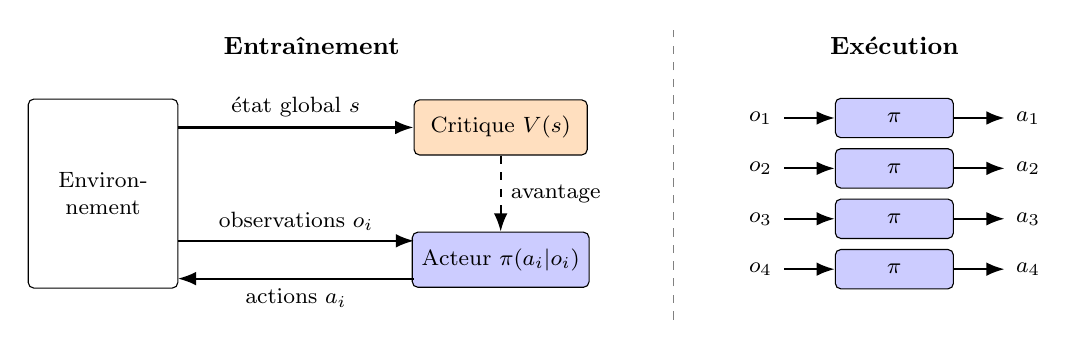
\begin{tikzpicture}[
      y=0.8cm,
      font=\footnotesize,
      box/.style={draw,rounded corners=2pt,align=center,minimum height=0.7cm,minimum width=2.2cm},
      flow/.style={-{Latex},thick}
    ]
    \node[font=\small\bfseries] at (3.6,2.35) {Entraînement};
    \node[box,minimum height=2.4cm,minimum width=1.9cm] (env) at (0.95,0) {Environ-\\nement};
    \node[box,fill=orange!25] (critic) at (6,1.05) {Critique $V(s)$};
    \node[box,fill=blue!20] (actor) at (6,-1.05) {Acteur $\pi(a_i|o_i)$};
    \draw[flow] (1.9,1.05) -- node[above] {état global $s$} (critic.west);
    \draw[flow] (1.9,-0.75) -- node[above] {observations $o_i$} (4.9,-0.75);
    \draw[flow] (4.9,-1.35) -- node[below] {actions $a_i$} (1.9,-1.35);
    \draw[flow,dashed] (critic.south) -- node[right] {avantage} (actor.north);

    \draw[dashed,gray] (8.2,-2) -- (8.2,2.6);

    \node[font=\small\bfseries] at (11,2.35) {Exécution};
    \foreach \i/\y in {1/1.2,2/0.4,3/-0.4,4/-1.2} {
      \node at (9.3,\y) {$o_\i$};
      \node[draw,rounded corners=2pt,fill=blue!20,minimum width=1.5cm,minimum height=0.5cm] (p\i) at (11,\y) {$\pi$};
      \node at (12.7,\y) {$a_\i$};
      \draw[flow] (9.6,\y) -- (p\i.west);
      \draw[flow] (p\i.east) -- (12.4,\y);
    }
  \end{tikzpicture}

  \vfill
  \raggedright
  {\scriptsize\setlength{\parskip}{0pt}
    [1] Yu et al., \emph{The Surprising Effectiveness of PPO in Cooperative Multi-Agent Games}, arXiv:2103.01955.\par
    [2] Lowe et al., \emph{Multi-Agent Actor-Critic for Mixed Cooperative-Competitive Environments}, NeurIPS 2017.\par}
\end{frame}

\begin{frame}{Ce que voit la critique : toute la grille}
  \begin{columns}[c]
    \column{0.52\textwidth}
    \centering
    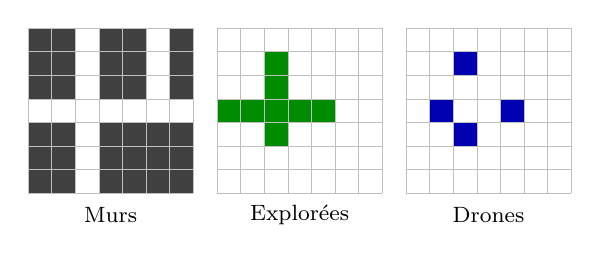
\begin{tikzpicture}[scale=0.3]
      \fill[black!75] (0,0) rectangle (7,7);
      \foreach \x/\y in \tunnels {\fill[white] (\x,\y) rectangle ++(1,1);}
      \gridlines
      \node[font=\footnotesize] at (3.5,-0.9) {Murs};
      \begin{scope}[shift={(8,0)}]
        \foreach \x/\y in \exploredcells {\fill[green!55!black] (\x,\y) rectangle ++(1,1);}
        \gridlines
        \node[font=\footnotesize] at (3.5,-0.9) {Explorées};
      \end{scope}
      \begin{scope}[shift={(16,0)}]
        \foreach \x/\y in \dronecells {\fill[blue!70!black] (\x,\y) rectangle ++(1,1);}
        \gridlines
        \node[font=\footnotesize] at (3.5,-0.9) {Drones};
      \end{scope}
    \end{tikzpicture}

    \column{0.46\textwidth}
    \small
    \begin{itemize}
      \item Image de toute la carte, 3 canaux : 56$\times$56$\times$3 pour une carte 50$\times$50
      \item Voit ce que l'équipe a exploré et tous les drones
      \item Possible : elle ne sert qu'à l'entraînement
      \item Avant : méthode plus compacte, MLP sur les 4 observations concaténées (148 valeurs)
    \end{itemize}
  \end{columns}
\end{frame}

\begin{frame}{Ce que voit l'acteur : son voisinage}
  \begin{columns}[c]
    \column{0.42\textwidth}
    \centering
    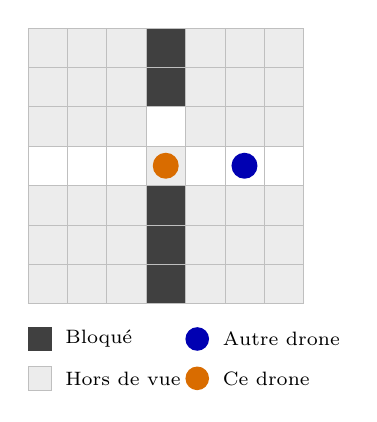
\begin{tikzpicture}[scale=0.5]
      \fill[gray!15] (0,0) rectangle (7,7);
      \foreach \x/\y in {3/4,2/3,1/3,0/3,4/3,5/3,6/3} {\fill[white] (\x,\y) rectangle ++(1,1);}
      \foreach \x/\y in {3/5,3/6,3/2,3/1,3/0} {\fill[black!75] (\x,\y) rectangle ++(1,1);}
      \fill[blue!70!black] (5.5,3.5) circle (0.33);
      \fill[orange!85!black] (3.5,3.5) circle (0.33);
      \draw[step=1,gray!50,very thin] (0,0) grid (7,7);
      \fill[black!75] (0,-1.2) rectangle ++(0.6,0.6);
      \node[anchor=west,font=\scriptsize] at (0.7,-0.9) {Bloqué};
      \fill[blue!70!black] (4.3,-0.9) circle (0.3);
      \node[anchor=west,font=\scriptsize] at (4.7,-0.9) {Autre drone};
      \fill[gray!15] (0,-2.2) rectangle ++(0.6,0.6);
      \draw[gray!50,very thin] (0,-2.2) rectangle ++(0.6,0.6);
      \node[anchor=west,font=\scriptsize] at (0.7,-1.9) {Hors de vue};
      \fill[orange!85!black] (4.3,-1.9) circle (0.3);
      \node[anchor=west,font=\scriptsize] at (4.7,-1.9) {Ce drone};
    \end{tikzpicture}

    \column{0.56\textwidth}
    \small
    \begin{itemize}
      \item 4 rayons de 3 cases pour : "Bloqué" et "Autre drone" ( $3\times 4 \times 2 = 24$ valeurs)
      \item MLP (256, 256) vers 5 actions, avec masque des actions impossibles
      \item Seul réseau utilisé à l'exécution
      \item Il ne voit pas les cases explorées : sans mémoire, un couloir neuf et un couloir visité sont identiques
    \end{itemize}
  \end{columns}

  \vfill
  {\footnotesize Ancienne version : les rayons indiquaient aussi les cases explorées, 36 valeurs au lieu de 24.}
\end{frame}

\begin{frame}{Les deux réseaux}
  \centering
  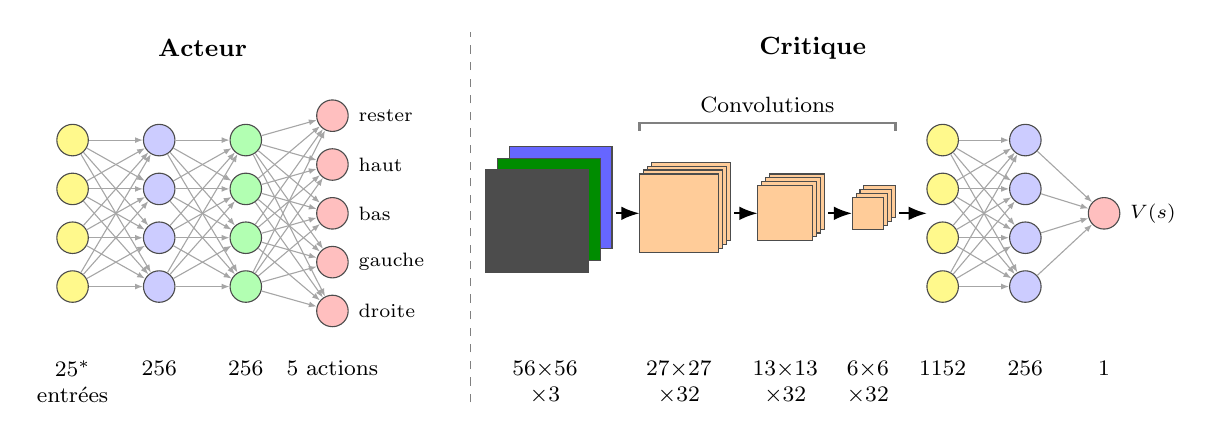
\begin{tikzpicture}
    \node[font=\small\bfseries] at (1.65,2.1) {Acteur};
    \nnlayer{a}{0}{4}{yellow!45}{25$^*$\\entrées}
    \nnlayer{b}{1.1}{4}{blue!20}{256}
    \nnlayer{c}{2.2}{4}{green!30}{256}
    \nnlayer{d}{3.3}{5}{red!25}{5 actions}
    \nnlink{a}{4}{b}{4}
    \nnlink{b}{4}{c}{4}
    \nnlink{c}{4}{d}{5}
    \foreach \t [count=\k] in {rester,haut,bas,gauche,droite} {\node[right,font=\scriptsize] at (d\k.east) {\t};}

    \draw[dashed,gray] (5.05,-2.4) -- (5.05,2.3);

    \node[font=\small\bfseries] at (9.4,2.1) {Critique};
    \draw[fill=blue!60,draw=black!70,thin] (5.55,-0.45) rectangle ++(1.3,1.3);
    \draw[fill=green!55!black,draw=black!70,thin] (5.4,-0.6) rectangle ++(1.3,1.3);
    \draw[fill=black!70,draw=black!70,thin] (5.25,-0.75) rectangle ++(1.3,1.3);
    \node[font=\footnotesize,align=center,anchor=north] at (6,-1.75) {56$\times$56\\$\times$3};
    \fmap{7.7}{1}{27$\times$27\\$\times$32}
    \fmap{9.05}{0.7}{13$\times$13\\$\times$32}
    \fmap{10.1}{0.4}{6$\times$6\\$\times$32}
    \foreach \a/\b in {6.9/7.2,8.4/8.7,9.6/9.9,10.5/10.85} {\draw[-{Latex},thick] (\a,0) -- (\b,0);}
    \draw[thick,gray] (7.2,1.05) -- (7.2,1.15) -- node[above,font=\footnotesize,text=black] {Convolutions} (10.45,1.15) -- (10.45,1.05);
    \nnlayer{e}{11.05}{4}{yellow!45}{1152}
    \nnlayer{f}{12.1}{4}{blue!20}{256}
    \nnlayer{g}{13.1}{1}{red!25}{1}
    \nnlink{e}{4}{f}{4}
    \nnlink{f}{4}{g}{1}
    \node[right,font=\scriptsize] at (g1.east) {$V(s)$};
  \end{tikzpicture}

  \vfill
  \raggedright
  {\footnotesize $^*$ 24 valeurs des rayons + 1 indicateur de case partagée.\par}
\end{frame}

\section{Modifications de l'environnement}

\begin{frame}{Plus de superposition entre drones}
  \begin{itemize}
    \item Avant : plusieurs drones pouvaient occuper la même case
    \item Maintenant : une case, un drone
    \item Seule exception : au départ, les 4 drones sont empilés sur la case de départ
  \end{itemize}

  \vspace{0.6em}
  \begin{columns}[T]
    \column{0.33\textwidth}
    \centering
    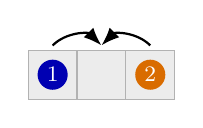
\begin{tikzpicture}[scale=0.62]
      \foreach \x in {0,1,2} {\cell{\x}}
      \drone{0}{1}{blue!70!black}
      \drone{2}{2}{orange!85!black}
      \moveR{0}{1}
      \moveL{2}{1}
    \end{tikzpicture}

    \small Même case visée :\\ tirage au sort, l'autre reste
    \column{0.33\textwidth}
    \centering
    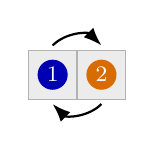
\begin{tikzpicture}[scale=0.62]
      \foreach \x in {0,1} {\cell{\x}}
      \drone{0}{1}{blue!70!black}
      \drone{1}{2}{orange!85!black}
      \moveR{0}{1}
      \moveB{1}{0}
    \end{tikzpicture}

    \small Échange de cases :\\ interdit, les deux restent
    \column{0.33\textwidth}
    \centering
    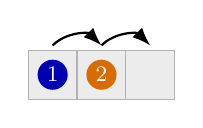
\begin{tikzpicture}[scale=0.62]
      \foreach \x in {0,1,2} {\cell{\x}}
      \drone{0}{1}{blue!70!black}
      \drone{1}{2}{orange!85!black}
      \moveR{1}{2}
      \moveR{0}{1}
    \end{tikzpicture}

    \small Case libérée au même step :\\ autorisé
  \end{columns}
\end{frame}

\begin{frame}{Autres changements}
  \begin{itemize}
    \item Patience : l'épisode s'arrête si l'équipe ne découvre rien pendant un nombre de steps égal au diamètre de la carte
    \item Évaluation : politique déterministe, chaque carte de validation jouée une fois
  \end{itemize}
\end{frame}

\section{Réglage de l'entraînement}

\begin{frame}{\texttt{n\_envs} et \texttt{frames\_per\_batch} : 2 cartes, 3M frames}
  \centering
  \small
  \begin{tabular}{rrrlrr}
    \toprule
    n\_envs & frames/batch & steps/env & device & temps & frames/s \\
    \midrule
    120 & 6\,000 & 50 & CPU & 303 s & 9\,900 \\
    1024 & 51\,200 & 50 & GPU & 151 s & 20\,300 \\
    4096 & 204\,800 & 50 & GPU & 160--180 s & 17--19\,000 \\
    \bottomrule
  \end{tabular}

  \vspace{0.8em}
  \raggedright
  \normalsize
  \begin{itemize}
    \item Le GPU double la vitesse, mais 4096 envs ne vont pas plus vite que 1024
  \end{itemize}
\end{frame}

\section{Génération de cartes}

\begin{frame}{Trois jeux de cartes séparés}
  \centering
  \begin{tabular}{llp{8.2cm}}
    \toprule
    Jeu & Cartes & Utilisation \\
    \midrule
    train & 73 & Entraînement, une carte tirée au hasard à chaque reset \\
    val & 14 & Évaluation pendant l'entraînement, réglage des hyperparamètres et de la récompense \\
    test & 16 & Évaluation finale uniquement, jamais pour régler quoi que ce soit \\
    \bottomrule
  \end{tabular}

  \vspace{0.8em}
  \raggedright
  \begin{itemize}
    \item train et val : 7 familles, cartes 50$\times$50, 2 cartes de chaque famille en val
    \item test : 8 cartes issues des familles et 8 cartes de catégories jamais vues, de 12$\times$12 à 100$\times$100
  \end{itemize}
\end{frame}

\begin{frame}{Les 7 familles (train et val)}
  \centering
  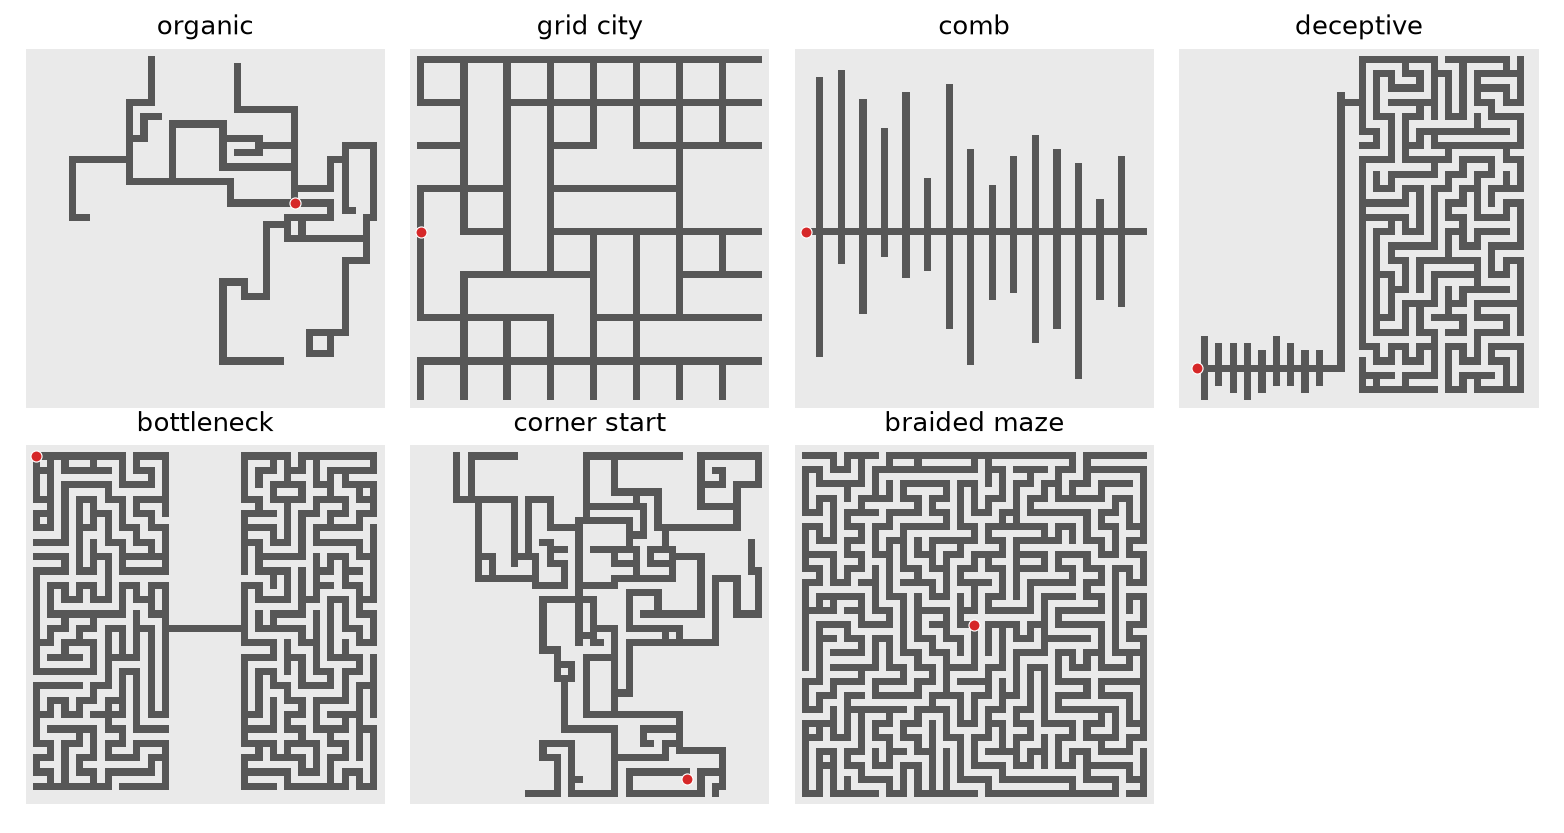
\includegraphics[height=0.84\textheight]{maps_families}
\end{frame}

\begin{frame}{Les 8 catégories présentes uniquement en test}
  \centering
  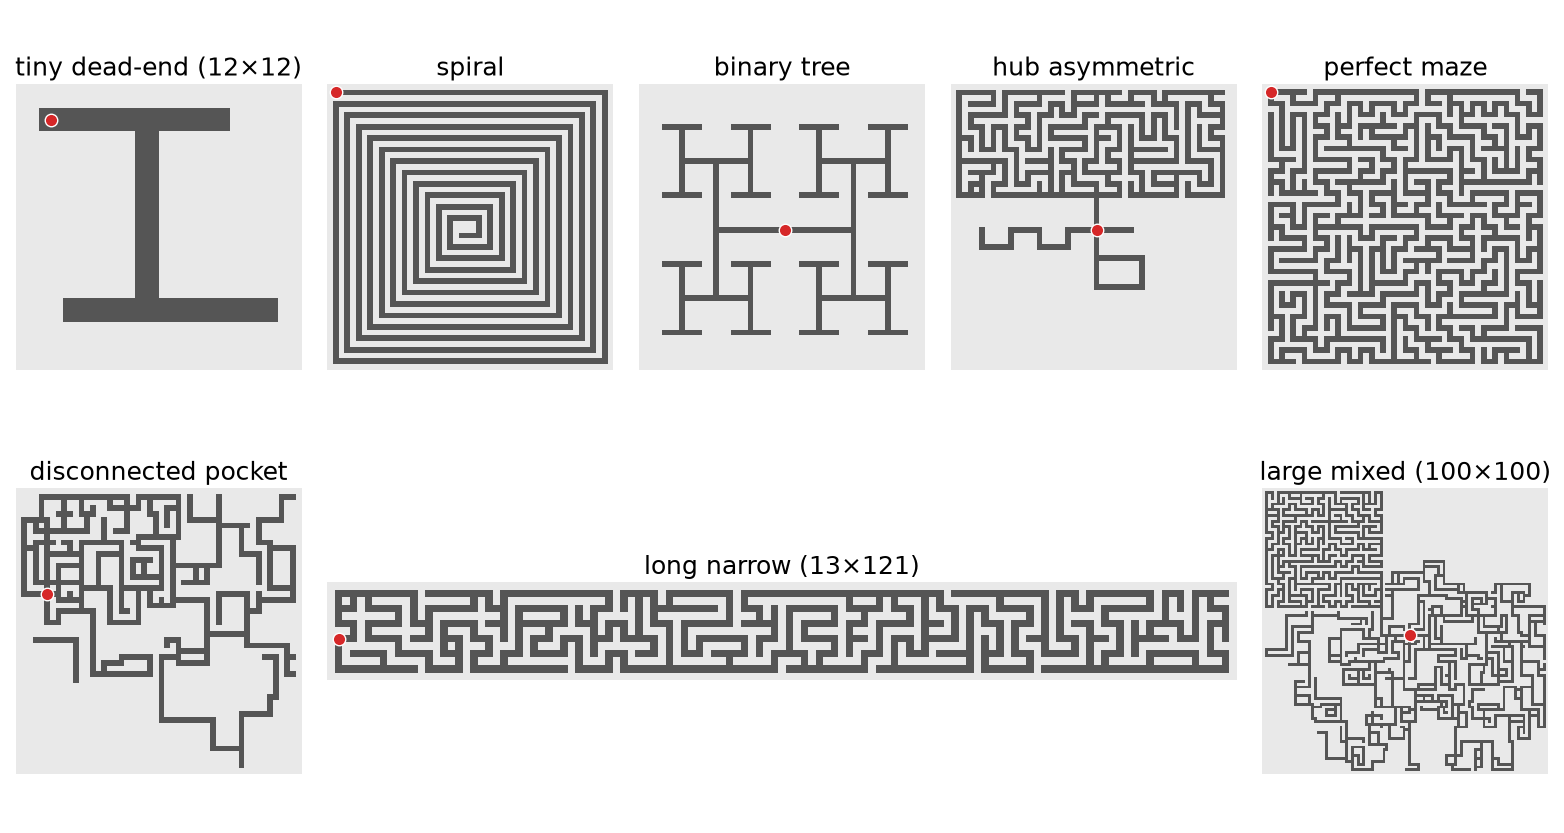
\includegraphics[height=0.84\textheight]{maps_test_only}
\end{frame}

\section{Hot vector}

\begin{frame}{Donner une identité à chaque drone}
  \begin{itemize}
    \item Politique partagée et même observation donnent la même action
    \item Au départ, les 4 drones sont sur la même case et voient la même chose
    \item Ajout de l'identifiant du drone en one-hot à la fin de l'observation
    \item Objectif : permettre à chaque drone d'apprendre un rôle différent
  \end{itemize}

  \centering
  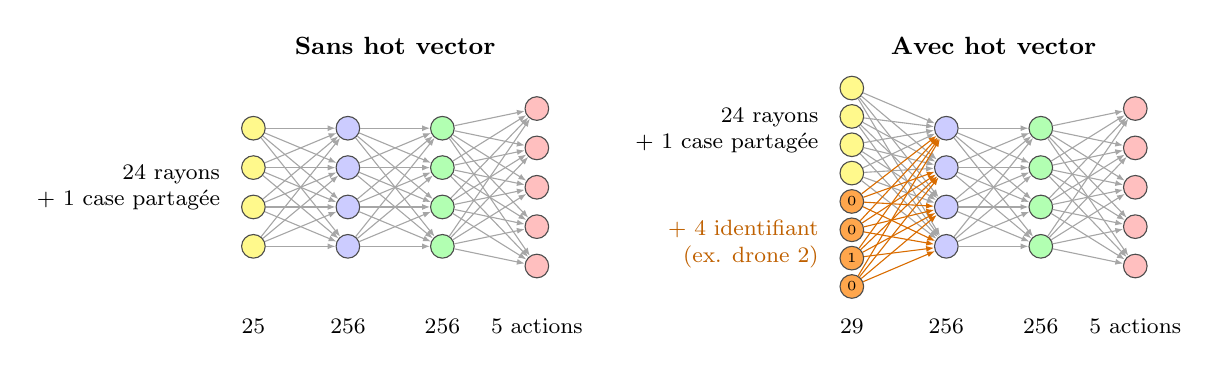
\begin{tikzpicture}
    \node[font=\small\bfseries] at (1.8,1.8) {Sans hot vector};
    \foreach \k in {1,...,4} {\node[neuronS,fill=yellow!45] (na\k) at (0,{(2.5-\k)*0.5}) {};}
    \hvbody{n}
    \foreach \a in {1,...,4} {\foreach \b in {1,...,4} {\draw[-{Latex[length=1mm]},gray!70,thin] (na\a) -- (nb\b);}}
    \node[font=\footnotesize,align=right,anchor=east] at (-0.3,0) {24 rayons\\+ 1 case partagée};
    \node[font=\footnotesize,align=center,anchor=north] at (0,-1.55) {25};

    \begin{scope}[xshift=7.6cm]
      \node[font=\small\bfseries] at (1.8,1.8) {Avec hot vector};
      \foreach \k in {1,...,4} {\node[neuronS,fill=yellow!45] (ha\k) at (0,{(4.5-\k)*0.36}) {};}
      \foreach \k/\v in {5/0,6/0,7/1,8/0} {\node[neuronS,fill=orange!70] (ha\k) at (0,{(4.5-\k)*0.36}) {\v};}
      \hvbody{h}
      \foreach \a in {1,...,4} {\foreach \b in {1,...,4} {\draw[-{Latex[length=1mm]},gray!70,thin] (ha\a) -- (hb\b);}}
      \foreach \a in {5,...,8} {\foreach \b in {1,...,4} {\draw[-{Latex[length=1mm]},orange!85!black,thin] (ha\a) -- (hb\b);}}
      \node[font=\footnotesize,align=right,anchor=east] at (-0.3,0.72) {24 rayons\\+ 1 case partagée};
      \node[font=\footnotesize,align=right,anchor=east,text=orange!75!black] at (-0.3,-0.72) {+ 4 identifiant\\(ex. drone 2)};
      \node[font=\footnotesize,align=center,anchor=north] at (0,-1.55) {29};
    \end{scope}
  \end{tikzpicture}
\end{frame}

\section{Bilan des deux approches}

\begin{frame}{Bilan des deux approches}
  \begin{columns}[c]
    \column{0.55\textwidth}
    \footnotesize
    \setlength{\parskip}{2pt}
    \textbf{Ancienne version}
    \begin{itemize}\setlength{\itemsep}{1pt}
      \item Critique compacte : 4 observations concaténées
      \item Acteur : voit les cases explorées par toute l'équipe
      \item Couverture autour de 30 \% 
      \item Hot vector : gain léger et irrégulier
      \item Stigmergie : peu praticable dans un tunnel
    \end{itemize}

    \textbf{Approche actuelle}
    \begin{itemize}\setlength{\itemsep}{1pt}
      \item Conditions décrites dans les slides précédentes
      \item Plus lent, résultats moins bons, mais bonne entropie
    \end{itemize}
    \column{0.43\textwidth}
    \centering
    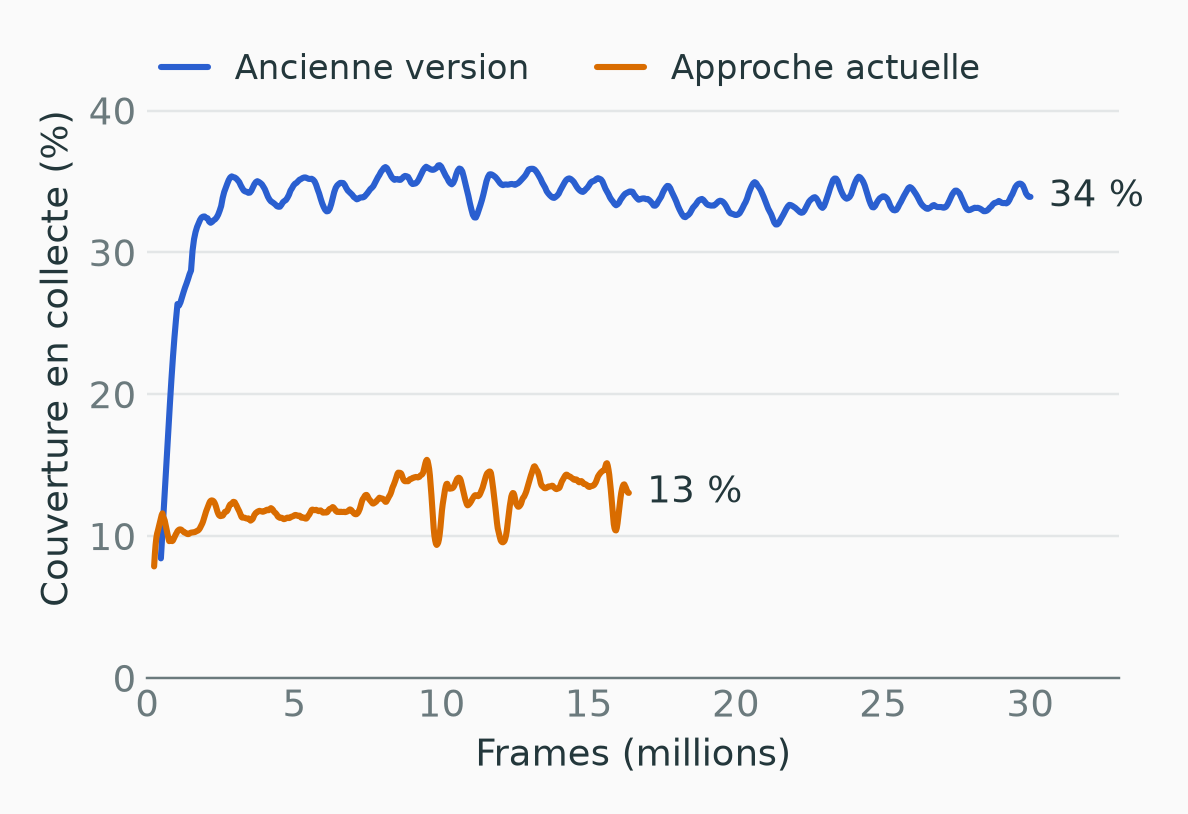
\includegraphics[width=0.78\linewidth]{coverage_approches}

    \vspace{0.3em}
    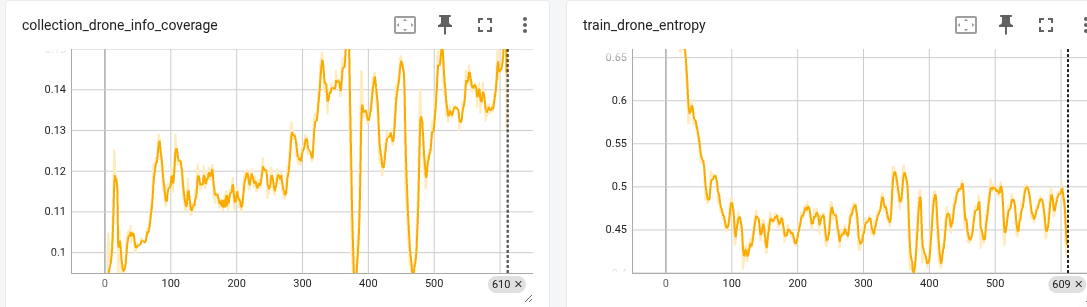
\includegraphics[width=\linewidth]{tensorboard_approche_actuelle}
  \end{columns}
\end{frame}

\section{Conclusion}

\begin{frame}{Suite du travail}
  \begin{enumerate}
    \item Pousser au maximum l'approche actuelle : donner le moins d'information possible à l'acteur (pas de mémoire, view range limité)
    \begin{itemize}
      \item Modifier le coefficient d'entropie (0 actuellement)
      \item Récompense personnalisée (mode \texttt{mixed})
    \end{itemize}
    \vspace{0.6em}
    \item Partager entre les agents la carte connue individuellement ?
  \end{enumerate}
\end{frame}

\begin{frame}{Protocole d'expérimentation et de validation}
  Pour évaluer les résultats, nous devrons décider :

  \vspace{0.6em}
  \centering
  \small
  \renewcommand{\arraystretch}{1.35}
  \begin{tabular}{p{2.9cm}p{9.8cm}}
    \toprule
    À décider & Propositions (à faire évoluer) \\
    \midrule
    Métriques & Couverture finale, steps pour atteindre 50 \% et 90 \%, part d'épisodes terminés, recouvrement entre drones \\
    Références & Aléatoire, frontière (à implémenter), Wall Follower, Trémaux, Edge Ant Walk \\
    Critères de réussite & Battre l'aléatoire sur toutes les familles\\
    \bottomrule
  \end{tabular}
\end{frame}

\end{document}
